%%%%%%%%%%%%%%%%%%%%%%%%%%%%%%%%%%%%%%%%%%%%%%%%%%%%%%%%%%%%%%%%%%%%%%%%%%%%%%%%%%%%%%%%%%%%%%%%%%%%%
% DOCUMENT CLASS
%%%%%%%%%%%%%%%%%%%%%%%%%%%%%%%%%%%%%%%%%%%%%%%%%%%%%%%%%%%%%%%%%%%%%%%%%%%%%%%%%%%%%%%%%%%%%%%%%%%%%%

% Single-spaced, two-column with PRL look and style (easy on the eyes)
\documentclass[aps,prl,twocolumn,superscriptaddress,floatfix]{revtex4-1}

% Double-spaced, one-column style (for submission/review/editing)
%\documentclass[aps,preprint,prl,superscriptaddress,showpacs]{revtex4}

%%%%%%%%%%%%%%%%%%%%%%%%%%%%%%%%%%%%%%%%%%%%%%%%%%%%%%%%%%%%%%%%%%%%%%%%%%%%%%%%%%%%%%%%%%%%%%%%%%%%%%
% PREAMBLE
%%%%%%%%%%%%%%%%%%%%%%%%%%%%%%%%%%%%%%%%%%%%%%%%%%%%%%%%%%%%%%%%%%%%%%%%%%%%%%%%%%%%%%%%%%%%%%%%%%%%%%

\usepackage{palatino}
\usepackage{amsmath}
\usepackage{amssymb}
\usepackage{graphicx}
\usepackage{dcolumn}
\usepackage{boxedminipage}
\usepackage{verbatim}
\usepackage[colorlinks=true,citecolor=blue,linkcolor=blue]{hyperref}

% The figures are in a figures/ subdirectory.
\graphicspath{{../figures/}}

% italicized boldface for math (e.g. vectors)
\newcommand{\bfv}[1]{{\mbox{\boldmath{$#1$}}}}
% non-italicized boldface for math (e.g. matrices)
\newcommand{\bfm}[1]{{\bf #1}}          

%\newcommand{\bfm}[1]{{\mbox{\boldmath{$#1$}}}}
%\newcommand{\bfm}[1]{{\bf #1}}
\newcommand{\expect}[1]{\left \langle #1 \right \rangle}                % <.> for denoting expectations over realizations of an experiment or thermal averages

% vectors
\newcommand{\x}{\bfv{x}}
\newcommand{\y}{\bfv{y}}
\newcommand{\f}{\bfv{f}}

\newcommand{\bfc}{\bfm{c}}
\newcommand{\hatf}{\hat{f}}

\newcommand{\bTheta}{\bfm{\Theta}}
\newcommand{\btheta}{\bfm{\theta}}
\newcommand{\bhatf}{\bfm{\hat{f}}}
\newcommand{\Cov}[1] {\mathrm{cov}\left( #1 \right)}
\newcommand{\Ept}[1] {{\mathrm E}\left[ #1 \right]}
\newcommand{\Eptk}[2] {{\mathrm E}_{#1}\left[ #2\right]}
\newcommand{\T}{\mathrm{T}}                                % T used in matrix transpose

\begin{document}

%%%%%%%%%%%%%%%%%%%%%%%%%%%%%%%%%%%%%%%%%%%%%%%%%%%%%%%%%%%%%%%%%%%%%%%%%%%%%%%%%%%%%%%%%%%%%%%%%%%%%%
% TITLE AND AUTHORS
%%%%%%%%%%%%%%%%%%%%%%%%%%%%%%%%%%%%%%%%%%%%%%%%%%%%%%%%%%%%%%%%%%%%%%%%%%%%%%%%%%%%%%%%%%%%%%%%%%%%%%

%\title{When is extension a good reaction coordinate in single-molecule pulling experiments?}
\title{Supplementary material for\\
``Splitting probabilities as a test of reaction coordinate choice in single-molecule experiments''}

 \author{John D. Chodera}
 \email{jchodera@berkeley.edu}
 \affiliation{California Institute of Quantitative Biosciences (QB3), University of California, Berkeley, CA 94720}
 
\author{Vijay S. Pande}
 \thanks{Corresponding author}
  \email{pande@stanford.edu}
 \affiliation{Department of Chemistry, Stanford University, Stanford, CA 94305}

\date{\today}

%%%%%%%%%%%%%%%%%%%%%%%%%%%%%%%%%%%%%%%%%%%%%%%%%%%%%%%%%%%%%%%%%%%%%%%%%%%%%%%%%%%%%%%%%%%%%%%%%%%%%%
% ABSTRACT/pacs
%%%%%%%%%%%%%%%%%%%%%%%%%%%%%%%%%%%%%%%%%%%%%%%%%%%%%%%%%%%%%%%%%%%%%%%%%%%%%%%%%%%%%%%%%%%%%%%%%%%%%%

%\begin{abstract}
%Rapid developments in single-molecule techniques now permit single biomolecules to be monitored at equilibrium.
%To explain the observed dynamics, the experimentally-resolved observable is often chosen as a putative reaction coordinate along which kinetic behavior is presumed to be diffusive dynamics in the presence of free energy barriers.
%Here, we invoke the \emph{splitting probability} as a test of the suitability of a proposed reaction coordinate.
%Comparison of the observed splitting probability with that computed from the kinetic model provides a simple test to reject poor reaction coordinates.
%We demonstrate this test for a force spectroscopy measurement of a DNA hairpin.
%\end{abstract}
%
%\pacs{PACS codes go here}

\maketitle
\small
%%%%%%%%%%%%%%%%%%%%%%%%%%%%%%%%%%%%%%%%%%%%%%%%%%%%%%%%%%%%%%%%%%%%%%%%%%%%%%%%%%%%%%%%%%%%%%%%%%%%%%
% EMPIRICAL SPLITTING PROBABILITIES
%%%%%%%%%%%%%%%%%%%%%%%%%%%%%%%%%%%%%%%%%%%%%%%%%%%%%%%%%%%%%%%%%%%%%%%%%%%%%%%%%%%%%%%%%%%%%%%%%%%%%%

\section{Empirical splitting probability computation}

Computation of the empirical splitting probability $\hat{p}_A(x)$ (defined in Eq.~3 of the main text) along with associated statistical error $\delta \hat{p}_A(x)$ proceeded using the following scheme based on timeseries autocorrelation analysis~\cite{swope:1982a,janke:2002a}.
First, the observed range of $x$ seen in the discrete-time trajectory $x_t \equiv x(n\Delta t)$ was computed as $[x_\mathrm{min},x_\mathrm{max}]$, and this interval was split into 100 histogram bins of equal width.
A histogram function $\phi_i(x)$ was defined for each bin, assuming the value of unity if $x$ is in bin $i$, and zero otherwise.
For each bin $i$, two new timeseries are defined:
\begin{eqnarray}
a_t &\equiv& \phi_i(x_t) \, c_A(t) \nonumber \\
b_t &\equiv& \phi_i(x_t)
\end{eqnarray}
where $c_A(t)$ is the discrete-time analog of the hitting function defined in Eq.~5 of the main text.

The means of the new timeseries were computed:
\begin{eqnarray}
\hat{A} \equiv \frac{1}{T} \sum_{t=1}^T a_t \:\:;\:\: \hat{B} &\equiv& \frac{1}{T} \sum_{t=1}^T b_t 
\end{eqnarray}
and the sample covariances
\begin{eqnarray}
\hat{\sigma}^2_A &\equiv& \frac{1}{T} \sum_{t=1}^T (a_t - \hat{A})^2 \nonumber \\
\hat{\sigma}^2_B &\equiv& \frac{1}{T} \sum_{t=1}^T (b_t - \hat{B})^2 \nonumber \\
\hat{\sigma}^2_{AB} &\equiv& \frac{1}{T} \sum_{t=1}^T (a_t - \hat{A}) (b_t - \hat{B})
\end{eqnarray}
from which the squared statistical errors were computed
\begin{eqnarray}
\delta^2 \hat{A} &\equiv& \frac{\hat{\sigma}^2_A}{T / g_{A}} \nonumber \\
\delta^2 \hat{B} &\equiv& \frac{\hat{\sigma}^2_B}{T / g_{B}} \nonumber \\
\delta \hat{A} \delta \hat{B} &\equiv& \frac{\hat{\sigma}^2_{AB}}{T / g_{A;B}}
\end{eqnarray}
where the statistical inefficiencies $g_A$, $g_B$, and $g_{A;B}$ were computed as described in Ref.~\cite{chodera:jctc:2007}. 

Finally, the empirical splitting probability $\hat{p}_A(x)$ and the statistical uncertainty $\delta \hat{p}_A(x)$ for bin $i$ are computed using standard propagation of error (as in Ref.~\cite{chodera:jctc:2007}), obtaining 
\begin{eqnarray}
\hat{p}_A(x) &=& \frac{\hat{A}}{\hat{B}} \nonumber \\
\delta \hat{p}_A(x) &=& \left[ \frac{\hat{A}}{\hat{B}} \right]^2 \left[ \frac{\delta^2 \hat{A}}{\hat{A}^2} + \frac{\delta^2 \hat{B}}{\hat{B}^2} - 2 \frac{\delta \hat{A} \delta \hat{B}}{\hat{A} \hat{B}} \right]
\end{eqnarray}

Complete trajectories, histograms, estimated PMFs, and empirical and PMF-derived splitting probabilities for the model system data are shown in Supplementary Fig.~\ref{figure:model-trajectories}.

\begin{figure*}[tbp]
\resizebox{\textwidth}{!}{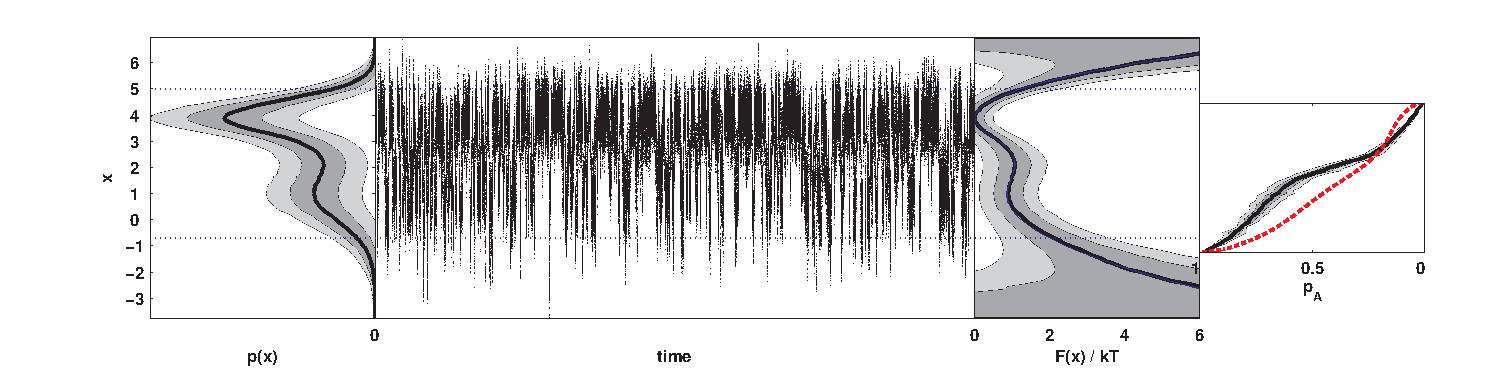
\includegraphics{rhee-pande-full_committor-x.pdf}}
\resizebox{\textwidth}{!}{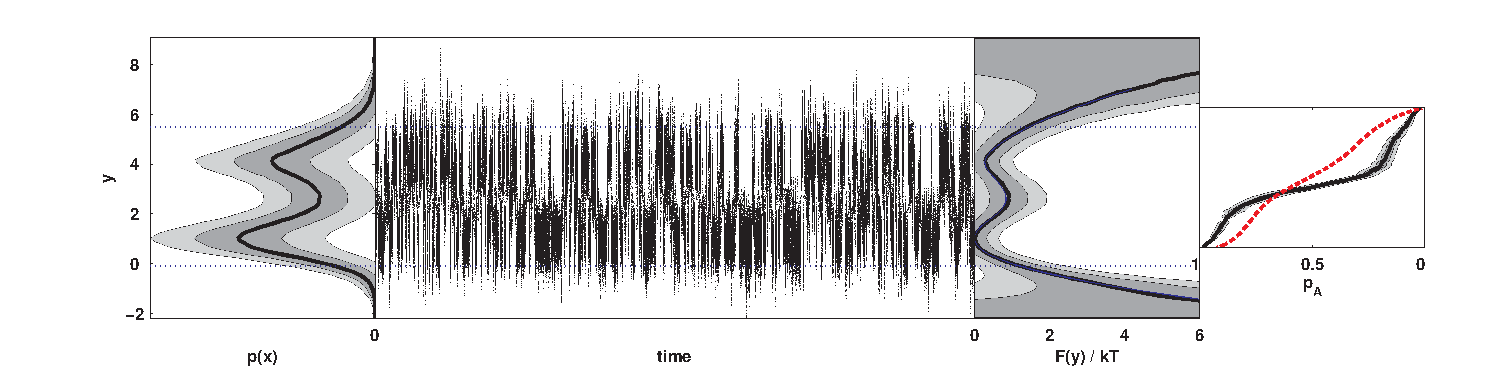
\includegraphics{rhee-pande-full_committor-y.pdf}}
\resizebox{\textwidth}{!}{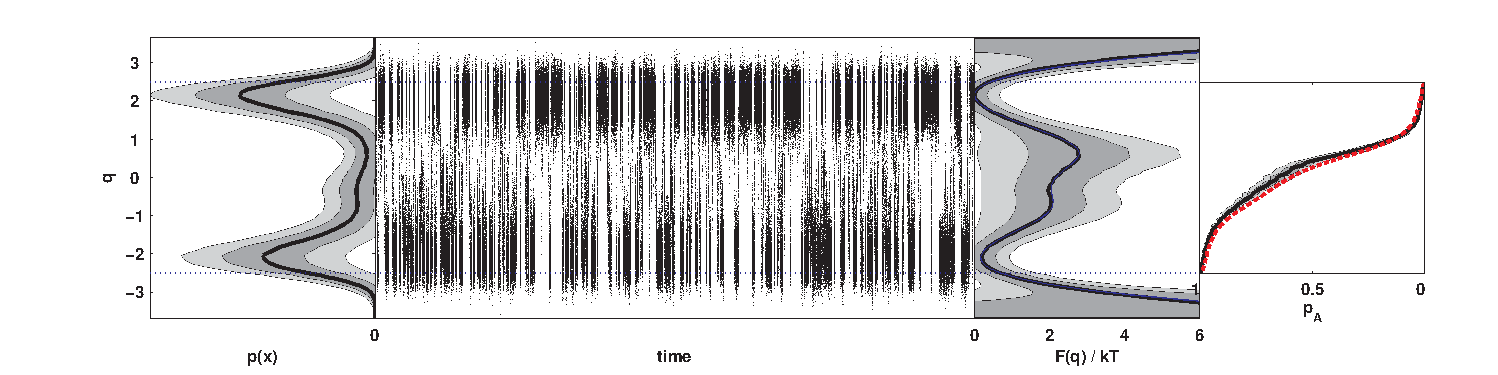
\includegraphics{rhee-pande-full_committor-q.pdf}}
\caption{\label{figure:model-splitting-comparison} {\bf Splitting probability tests for poor and good choices of reaction coordinate in two-dimensional model system.}
Splitting probability analysis for poor (top and middle) and good (bottom) choices of reaction coordinate for the two-dimensional model system depicted in Fig.~1 of the main text.
For each figure, the observed trajectory is shown in the large middle panel, with the observed histogram $p(x)$ and derived potential of mean force $F(x)$ flanking it to the left and right, respectively. 
The rightmost panel shows the coordinate-dependent average splitting probability $p_A(x)$ computed from the PMF and diffusion profile (red dashed line) and empirically estimated from the observed trajectory (black solid line).
For all computed quantities, dark black lines represent expectations, dark shading represents a 68\% confidence interval, and light shading a 95\% confidence interval.
}
\label{figure:model-trajectories}
\end{figure*}

%%%%%%%%%%%%%%%%%%%%%%%%%%%%%%%%%%%%%%%%%%%%%%%%%%%%%%%%%%%%%%%%%%%%%%%%%%%%%%%%%%%%%%%%%%%%%%%%%%%%%%
% COORDINATE-DEPENDENT DIFFUSION
%%%%%%%%%%%%%%%%%%%%%%%%%%%%%%%%%%%%%%%%%%%%%%%%%%%%%%%%%%%%%%%%%%%%%%%%%%%%%%%%%%%%%%%%%%%%%%%%%%%%%%

\section{Coordinate-dependent diffusion}

To compute position-dependent diffusion constants, the scheme of Best and Hummer was used~\cite{best-hummer:2010:pnas:coordinate-dependent-diffusion}.
The region in between absorbing boundary conditions was discretized into 50 bins of equal size in the corresponding coordinate, and an initial guess at the rate matrix made.
The number of statistically independent transition counts $N_{ij}$ between each pair of bins $i$ and $j$ for an observation interval of one sampling time was computed by dividing the total number of observed transitions in the trajectory $x_t$, $t = 0,\ldots,T$, by the statistical inefficiency $g_i$ of the timeseries of the corresponding indicator function for histogram bin $i$,
\begin{eqnarray}
b^{(i)}_t &\equiv& \phi_i(x_t) \:\:,\:\: t = 0,\ldots,T
\end{eqnarray}

The Bayesian posterior was then sampled from by choosing to perturb either $K_{i,i+1}$ or $K_{i,i-1}$ with equal probability.
Perturbations were of the form
\begin{eqnarray}
K'_{ij} &=& K_{ij} e^{(2 \Delta - 1)} \nonumber \\
K_{ii} &=& K_{ii} + K_{ij} - K'_{ij}
\end{eqnarray}
where $\Delta$ is a random number drawn uniformly on the interval $[0,1]$.
An initial 20 000 sampling iterations were discarded to burn-in, followed by another 20 000 production sampling iterations, with samples stored every 1 000 iterations.

For each transition matrix sample $\bfm{K}$, the potential of mean force and diffusion constant were computed as describes in Ref.~\cite{best-hummer:2010:pnas:coordinate-dependent-diffusion},
\begin{eqnarray}
F_i &=& - k_B T \ln \frac{\pi_i}{\delta x}  \\
D_i &=& \frac{(\delta x)^2}{2} \left[ K_{(i-1)i} \left(\frac{\pi_{i-1}}{\pi_i}\right)^{1/2} +  K_{i(i+1)} \left(\frac{\pi_i}{\pi_{i+1}}\right)^{1/2} \right] \nonumber
\end{eqnarray}
where $\delta x$ is the histogram bin width and $p_i$ is the stationary probability distribution computed from $\bfm{T} \equiv e^{\bfm{K} \tau}$ such that $\pi^\T \bfm{T} = \pi^\T$.
We note that the diffusion constant $D_i$ is an interpolation of the diffusion constants $D_{i-1/2}$ and $D_{i+1/2}$ defined in Ref.~\cite{best-hummer:2010:pnas:coordinate-dependent-diffusion}, in order to provide an estimate of the diffusion constant in bin $i$.
For each sampled set of $\{F_i, D_i\}$, the splitting probability was computed using Eq.~2 of the main text.

This analysis was performed for both the model system described in the main text (results shown in Supplementary Fig.~\ref{figure:coordinate-dependent-diffusion-model}) and the DNA hairpin data described in the main text (Supplementary Fig.~\ref{figure:coordinate-dependent-diffusion-hairpin}, with some panels reproduced in the main text as Fig.~4).

\begin{figure*}[tbp]
\resizebox{0.32\textwidth}{!}{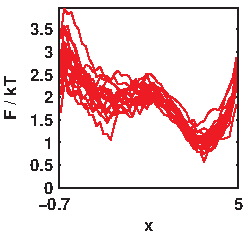
\includegraphics{pmf-x.pdf}}
\resizebox{0.32\textwidth}{!}{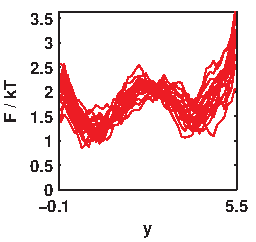
\includegraphics{pmf-y.pdf}}
\resizebox{0.32\textwidth}{!}{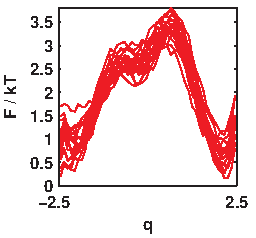
\includegraphics{pmf-q.pdf}}

\resizebox{0.32\textwidth}{!}{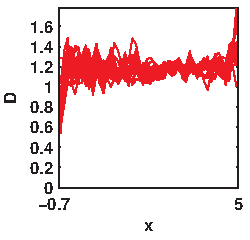
\includegraphics{diffusion-x.pdf}}
\resizebox{0.32\textwidth}{!}{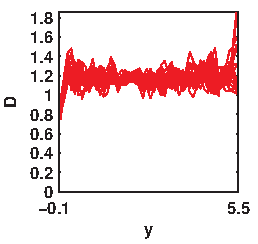
\includegraphics{diffusion-y.pdf}}
\resizebox{0.32\textwidth}{!}{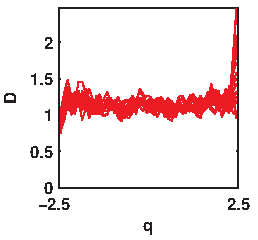
\includegraphics{diffusion-q.pdf}}

\resizebox{0.32\textwidth}{!}{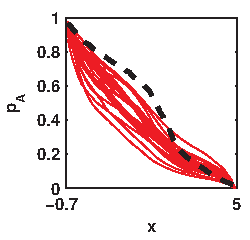
\includegraphics{best-hummer-x.pdf}}
\resizebox{0.32\textwidth}{!}{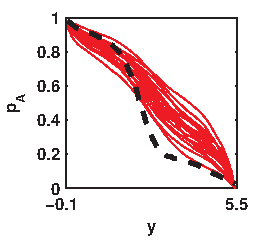
\includegraphics{best-hummer-y.pdf}}
\resizebox{0.32\textwidth}{!}{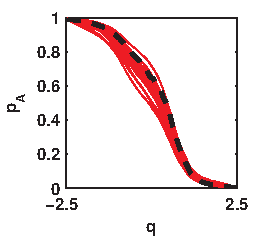
\includegraphics{best-hummer-q.pdf}}
\caption{{\bf Splitting probability tests for poor and good choices of reaction coordinate in two-dimensional model system, incorporating position-dependent diffusion.}
Splitting probability analysis for poor ($x$, left; $y$, middle) and good ($q$, right) choices of reaction coordinate for the two-dimensional model system depicted in Fig.~1 of the main text.
Red solid lines depict the 20 splitting probability profiles $p_A(s)$ computed from the PMFs and diffusion constants sampled from the Bayesian posterior, while the thick dashed black line depicts the empirical splitting probability profile $\hat{p}_A$.
}
\label{figure:coordinate-dependent-diffusion-model}
\end{figure*}

\begin{figure*}[tbp]
\resizebox{0.32\textwidth}{!}{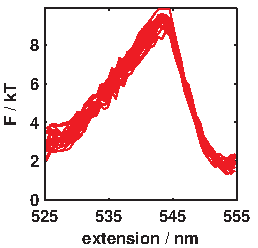
\includegraphics{pmf-extension.pdf}}
\resizebox{0.32\textwidth}{!}{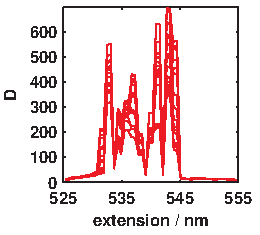
\includegraphics{diffusion-extension.pdf}}
\resizebox{0.32\textwidth}{!}{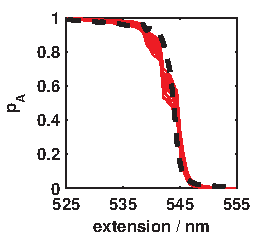
\includegraphics{best-hummer-extension.pdf}}
\caption{{\bf PMF, position-dependent diffusion constant, and splitting probability test incorporating position-dependent diffusion for DNA hairpin.}
All three plots were generated using the Best-Hummer Bayesian sampling scheme to sample the diffusion constant and PMF from the Bayesian posterior.
\emph{Left:} Potential of mean force (PMF) in extension coordinate, in nm.
\emph{Middle:} Position-dependent diffusion constant, in nm/s$^2$.
\emph{Right:} Splitting probability test in incorporating position-dependent diffusion constant, with red solid lines denoting the splitting probability $p_A$ computed from the PMF and diffusion constant, and the dashed black line denoting the empirical splitting probability $\hat{p}_A$.
}
\label{figure:coordinate-dependent-diffusion-hairpin}
\end{figure*}

%%%%%%%%%%%%%%%%%%%%%%%%%%%%%%%%%%%%%%%%%%%%%%%%%%%%%%%%%%%%%%%%%%%%%%%%%%%%%%%%%%%%%%%%%%%%%%%%%%%%%%
% BIBLIOGRAPHY
%%%%%%%%%%%%%%%%%%%%%%%%%%%%%%%%%%%%%%%%%%%%%%%%%%%%%%%%%%%%%%%%%%%%%%%%%%%%%%%%%%%%%%%%%%%%%%%%%%%%%%
\bibliography{single-molecule-pfold}


\end{document}